

\begin{landscape}
    \pagestyle{landscapestyle}
\section{Matriz de indicadores}
\begin{table}[H]
    \centering
    \includegraphics[width=1\linewidth]{indicators/images/indicadores1.png}
    \caption{Matriz de indicadores mes 1 - 6}
    \vspace{0.2cm}
    \small Fuente: Elaboración propia
    \label{tab:indicadores1}
\end{table}%

\begin{table}[H]
    \centering
    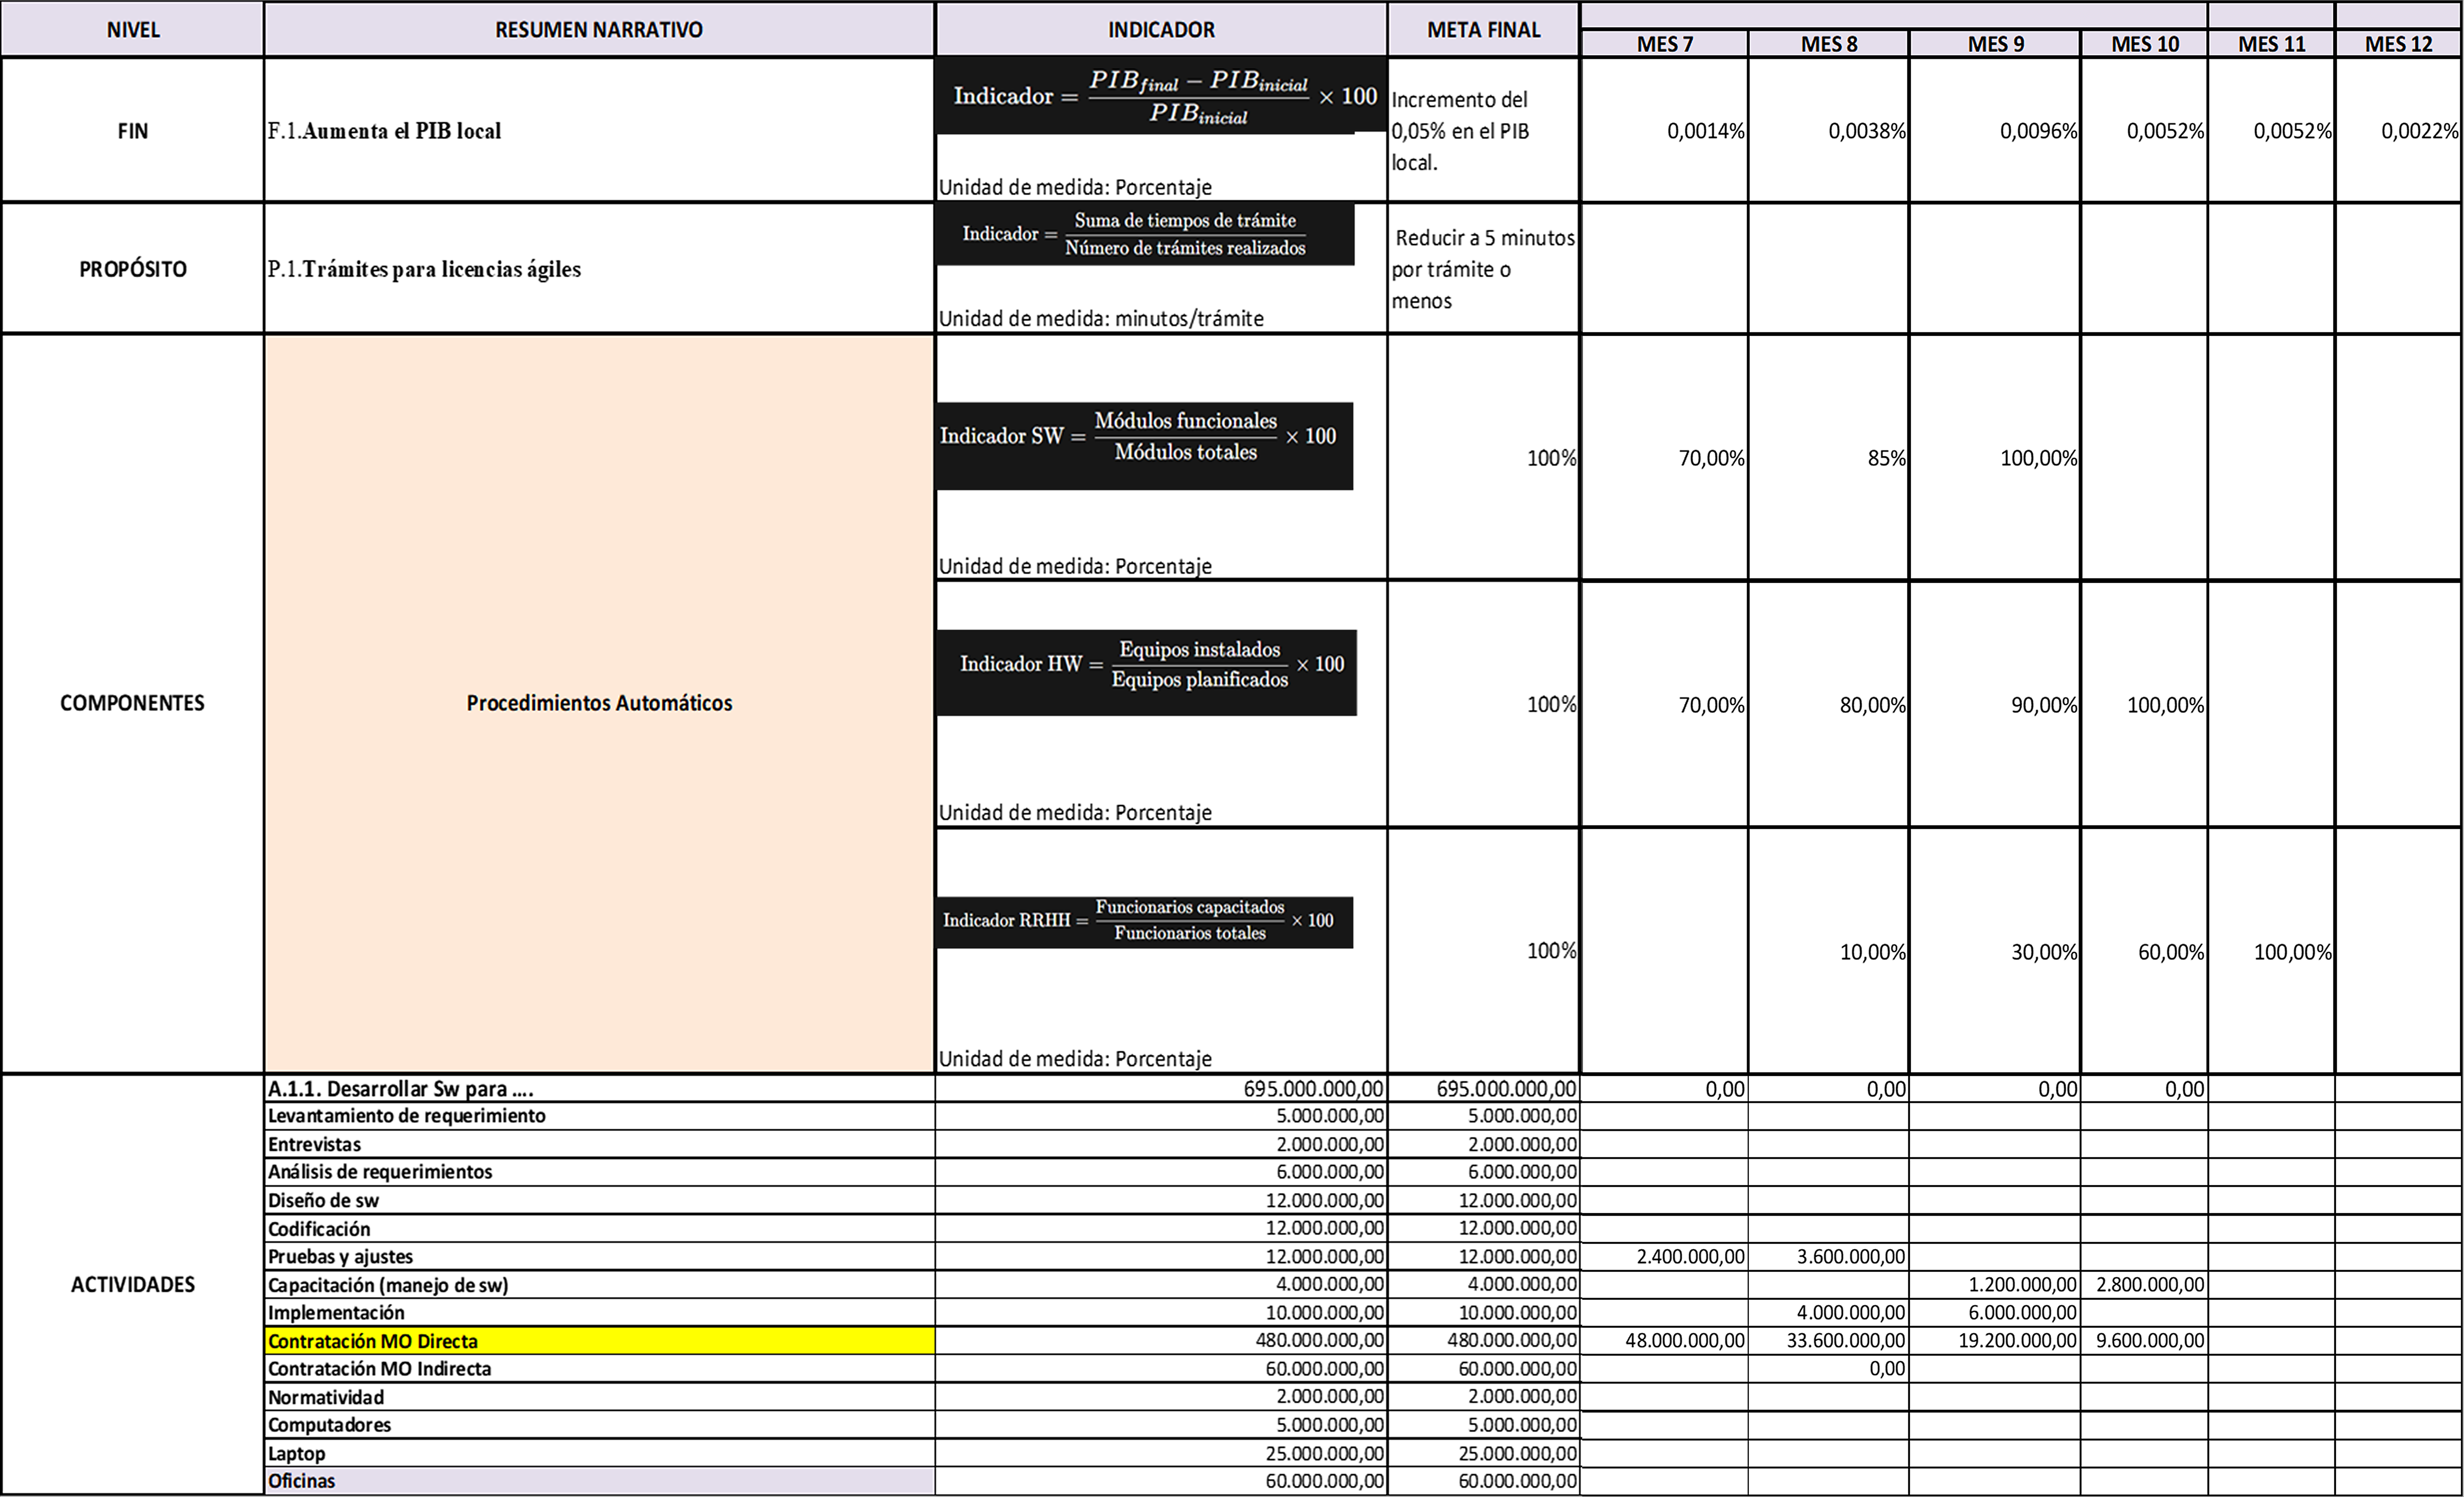
\includegraphics[width=1\linewidth]{indicators/images/indicadores2.png}
    \caption{Matriz de indicadores mes 7 - 12}
     \vspace{0.2cm}
    \small Fuente: Elaboración propia
    \label{tab:indicadores2}
\end{table}%
\end{landscape}

La implementación del sistema propuesto para la Secretaría de Tránsito de Pereira busca optimizar los procesos de expedición de licencias de conducción mediante la automatización de trámites. Este tipo de soluciones busca mejorar el crecimiento del Producto Interno Bruto (PIB) local, gracias a la reducción de costos operativos, el aumento de la productividad del personal y la disminución de tiempos de atención a los ciudadanos.

Diversos estudios internacionales respaldan la relación entre la digitalización del sector público y el crecimiento económico. De acuerdo con el Banco Interamericano de Desarrollo (BID, 2022), los proyectos de modernización digital en gobiernos locales de América Latina han generado aumentos en la productividad de entre 0,5\% y 0,8\% del PIB en un periodo de dos años. Por su parte, un estudio de \textit{McKinsey Global Institute} (McLKinsey, 2011) estimó que la digitalización de servicios públicos puede contribuir con hasta un 1,5\% anual al PIB de las economías en desarrollo. De manera similar, la \textit{OCDE} (OCDE, 2020) indicó que los procesos de transformación digital en instituciones gubernamentales generan incrementos sostenidos en la eficiencia económica entre 0,3\% y 1,0\% anual.

En el contexto colombiano, el DANE reportó que el PIB de Pereira alcanzó aproximadamente 28 billones de pesos en 2023 (DANE, 2024). Considerando esta base y los rangos de crecimiento derivados de la literatura mencionada, se estima que la implementación del sistema digital podría generar un impacto positivo progresivo sobre el PIB local equivalente a un aumento del 0,2\% durante el primer año y de 0,4\% en el segundo año.